%!TeX encoding = UTF-8
%!TeX program = xelatex
\documentclass[notheorems, aspectratio=54]{beamer}
% aspectratio: 1610, 149, 54, 43(default), 32
\usepackage[utf8]{inputenc}
\usepackage[vietnamese]{babel}
\usepackage{latexsym}
\usepackage{amsmath,amssymb}
\usepackage{mathtools}
\usepackage{color,xcolor}
\usepackage{graphicx}
\usepackage{algorithm}
\usepackage{amsthm}
\usepackage{lmodern} % 解决 font warning
% \usepackage[UTF8]{ctex}
\usepackage{animate} % insert gif

\usepackage{lipsum} % To generate test text 
\usepackage{ulem} % 下划线,波浪线

\usepackage{listings} % display code on slides; don't forget [fragile] option after \begin{frame}

% ----------------------------------------------
% tikx
\usepackage{framed}
\usepackage{tikz}
\usepackage{pgf}
\usetikzlibrary{calc,trees,positioning,arrows,chains,shapes.geometric,%
	decorations.pathreplacing,decorations.pathmorphing,shapes,%
	matrix,shapes.symbols}
\pgfmathsetseed{1} % To have predictable results
% Define a background layer, in which the parchment shape is drawn
\pgfdeclarelayer{background}
\pgfsetlayers{background,main}

% define styles for the normal border and the torn border
\tikzset{
	normal border/.style={orange!30!black!10, decorate, 
		decoration={random steps, segment length=2.5cm, amplitude=.7mm}},
	torn border/.style={orange!30!black!5, decorate, 
		decoration={random steps, segment length=.5cm, amplitude=1.7mm}}}

% Macro to draw the shape behind the text, when it fits completly in the
% page
\def\parchmentframe#1{
	\tikz{
		\node[inner sep=2em] (A) {#1};  % Draw the text of the node
		\begin{pgfonlayer}{background}  % Draw the shape behind
			\fill[normal border] 
			(A.south east) -- (A.south west) -- 
			(A.north west) -- (A.north east) -- cycle;
\end{pgfonlayer}}}

% Macro to draw the shape, when the text will continue in next page
\def\parchmentframetop#1{
	\tikz{
		\node[inner sep=2em] (A) {#1};    % Draw the text of the node
		\begin{pgfonlayer}{background}    
			\fill[normal border]              % Draw the ``complete shape'' behind
			(A.south east) -- (A.south west) -- 
			(A.north west) -- (A.north east) -- cycle;
			\fill[torn border]                % Add the torn lower border
			($(A.south east)-(0,.2)$) -- ($(A.south west)-(0,.2)$) -- 
			($(A.south west)+(0,.2)$) -- ($(A.south east)+(0,.2)$) -- cycle;
\end{pgfonlayer}}}

% Macro to draw the shape, when the text continues from previous page
\def\parchmentframebottom#1{
	\tikz{
		\node[inner sep=2em] (A) {#1};   % Draw the text of the node
		\begin{pgfonlayer}{background}   
			\fill[normal border]             % Draw the ``complete shape'' behind
			(A.south east) -- (A.south west) -- 
			(A.north west) -- (A.north east) -- cycle;
			\fill[torn border]               % Add the torn upper border
			($(A.north east)-(0,.2)$) -- ($(A.north west)-(0,.2)$) -- 
			($(A.north west)+(0,.2)$) -- ($(A.north east)+(0,.2)$) -- cycle;
\end{pgfonlayer}}}

% Macro to draw the shape, when both the text continues from previous page
% and it will continue in next page
\def\parchmentframemiddle#1{
	\tikz{
		\node[inner sep=2em] (A) {#1};   % Draw the text of the node
		\begin{pgfonlayer}{background}   
			\fill[normal border]             % Draw the ``complete shape'' behind
			(A.south east) -- (A.south west) -- 
			(A.north west) -- (A.north east) -- cycle;
			\fill[torn border]               % Add the torn lower border
			($(A.south east)-(0,.2)$) -- ($(A.south west)-(0,.2)$) -- 
			($(A.south west)+(0,.2)$) -- ($(A.south east)+(0,.2)$) -- cycle;
			\fill[torn border]               % Add the torn upper border
			($(A.north east)-(0,.2)$) -- ($(A.north west)-(0,.2)$) -- 
			($(A.north west)+(0,.2)$) -- ($(A.north east)+(0,.2)$) -- cycle;
\end{pgfonlayer}}}

% Define the environment which puts the frame
% In this case, the environment also accepts an argument with an optional
% title (which defaults to ``Example'', which is typeset in a box overlaid
% on the top border
\newenvironment{parchment}[1][Example]{%
	\def\FrameCommand{\parchmentframe}%
	\def\FirstFrameCommand{\parchmentframetop}%
	\def\LastFrameCommand{\parchmentframebottom}%
	\def\MidFrameCommand{\parchmentframemiddle}%
	\vskip\baselineskip
	\MakeFramed {\FrameRestore}
	\noindent\tikz\node[inner sep=1ex, draw=black!20,fill=white, 
	anchor=west, overlay] at (0em, 2em) {\sffamily#1};\par}%
{\endMakeFramed}

% ----------------------------------------------

\mode<presentation>{
	\usetheme{CambridgeUS}
	% Boadilla CambridgeUS
	% default Antibes Berlin Copenhagen
	% Madrid Montpelier Ilmenau Malmoe
	% Berkeley Singapore Warsaw
	\usecolortheme{beaver}
	% beetle, beaver, orchid, whale, dolphin
	\useoutertheme{infolines}
	% infolines miniframes shadow sidebar smoothbars smoothtree split tree
	\useinnertheme{circles}
	% circles, rectanges, rounded, inmargin
}
% 设置 block 颜色
\setbeamercolor{block title}{bg=red!30,fg=white}

\newcommand{\reditem}[1]{\setbeamercolor{item}{fg=red}\item #1}

% 缩放公式大小
\newcommand*{\Scale}[2][4]{\scalebox{#1}{\ensuremath{#2}}}

% 解决 font warning
\renewcommand\textbullet{\ensuremath{\bullet}}

% ---------------------------------------------------------------------
% flow chart
\tikzset{
	>=stealth',
	punktchain/.style={
		rectangle, 
		rounded corners, 
		% fill=black!10,
		draw=white, very thick,
		text width=6em,
		minimum height=2em, 
		text centered, 
		on chain
	},
	largepunktchain/.style={
		rectangle,
		rounded corners,
		draw=white, very thick,
		text width=10em,
		minimum height=2em,
		on chain
	},
	line/.style={draw, thick, <-},
	element/.style={
		tape,
		top color=white,
		bottom color=blue!50!black!60!,
		minimum width=6em,
		draw=blue!40!black!90, very thick,
		text width=6em, 
		minimum height=2em, 
		text centered, 
		on chain
	},
	every join/.style={->, thick,shorten >=1pt},
	decoration={brace},
	tuborg/.style={decorate},
	tubnode/.style={midway, right=2pt},
	font={\fontsize{10pt}{12}\selectfont},
}
% ---------------------------------------------------------------------

% code setting
\lstset{
	language=C++,
	basicstyle=\ttfamily\footnotesize,
	keywordstyle=\color{red},
	breaklines=true,
	xleftmargin=2em,
	numbers=left,
	numberstyle=\color[RGB]{222,155,81},
	frame=leftline,
	tabsize=4,
	breakatwhitespace=false,
	showspaces=false,               
	showstringspaces=false,
	showtabs=false,
	morekeywords={Str, Num, List},
}

% ---------------------------------------------------------------------
%
\author{\textbf{Nguyễn Hoàng Đức, Lê Nhựt Nam, Nguyễn Viết Dũng}\newline\newline
	GV Lý thuyết: \textbf{PGS. TS} Lê Hoàng Thái\newline
	GV Hướng dẫn: Nguyễn Ngọc Thảo, Lê Thanh Phong}
\title{SINH TRẮC HỌC GIỌNG NÓI\newline VOICE BIOMETRICS}

%
\setbeamertemplate{caption}[numbered]
% footer
\makeatletter
\setbeamertemplate{footline}
{
	\leavevmode%
	\hbox{%
		\begin{beamercolorbox}[wd=1\paperwidth,ht=2.25ex,dp=1ex,right]{institute in head/foot}%
			\usebeamerfont{title in head/foot} 
			\insertframenumber{} / \inserttotalframenumber\hspace*{2ex} 
	\end{beamercolorbox}}%
}
\makeatother

%
\newcommand{\argmax}{\arg\!\max}

\begin{document}

\begin{frame}
	\centering
	ĐẠI HỌC QUỐC GIA THÀNH PHỐ HỒ CHÍ MINH
	
	ĐẠI HỌC KHOA HỌC TỰ NHIÊN
	
	KHOA CÔNG NGHỆ THÔNG TIN - BỘ MÔN KHOA HỌC MÁY TÍNH
	\titlepage
\end{frame}
\begin{frame}{Nội dung trình bày}
	\textbf{A. Trình bày nội dung tìm hiểu được từ Chapter 8 - Voice Biometrics}
	\begin{itemize}
		\item Giới thiệu
		\item Xác định những thông tin trong tín hiệu giọng nói
		\item Rút trích đặc trưng và Phân tách dữ liệu
		\item Nhận dạng giọng nói phụ thuộc văn bản
		\item Nhận dạng giọng nói không phụ thuộc văn bản
		\item Ứng dụng
	\end{itemize}
\end{frame}
\begin{frame}{Nội dung trình bày}
	\textbf{B. Trình bày các phương pháp STATE OF THE ART của Voice Recognition}
	\begin{itemize}
		\item Mục đích
		\item Động lực nghiên cứu khoa học 
		\item Phát biểu bài toán
		\item Các công trình liên quan
		\item Phương pháp giải thuật
		\item Demo
		\item Tài liệu tham khảo
	\end{itemize}
\end{frame}

\section{Chapter 8 - Voice Biometrics}
\subsection{Giới thiệu về Sinh trắc học Giọng nói}
\begin{frame}{Giới thiệu}
	\begin{itemize}
		\item Giọng nói (Voice/Speech) là một đặc điểm sinh trắc học (nhân trắc học) dễ dàng tiếp cận nhất mà không cần phải có thêm thiết bị thu nhận và hệ thống truyền dẫn.
		\item Có lợi thế khi áp dụng vào các hệ thống điều khiển từ xa
		\item Giọng nói không chỉ liên quan đến các đặc trưng cá thể mà còn liên quan với môi trường xung quanh và vấn đề xã hội, do vậy việc sản sinh giọng nói là một kết quả của một quá trình hết sức phức tạp.
	\end{itemize}
\end{frame}
\subsection{Xác định những thông tin trong tín hiệu giọng nói}
\begin{frame}
	Những thông tin nhận dạng trong tín hiệu giọng nói
	\begin{itemize}
		\item Idiolectal characteristics: cách phát âm phản ánh khu vực bạn đang sống hoặc đã sống và các phong cách nói khác nhau thay đổi một cách tinh vi tùy thuộc vào người bạn đang nói đến.
		\item Phonotactics characteristics: 
		\item Prosody characteristics:
		\item Short-term spectral characteristics
	\end{itemize}
\end{frame}

\subsection{Rút trích đặc trưng và phân tách dữ liệu}
\begin{frame}{Phân tích theo từng đoạn ngắn (Short-term Analysis)}
	\begin{figure}[h!]
		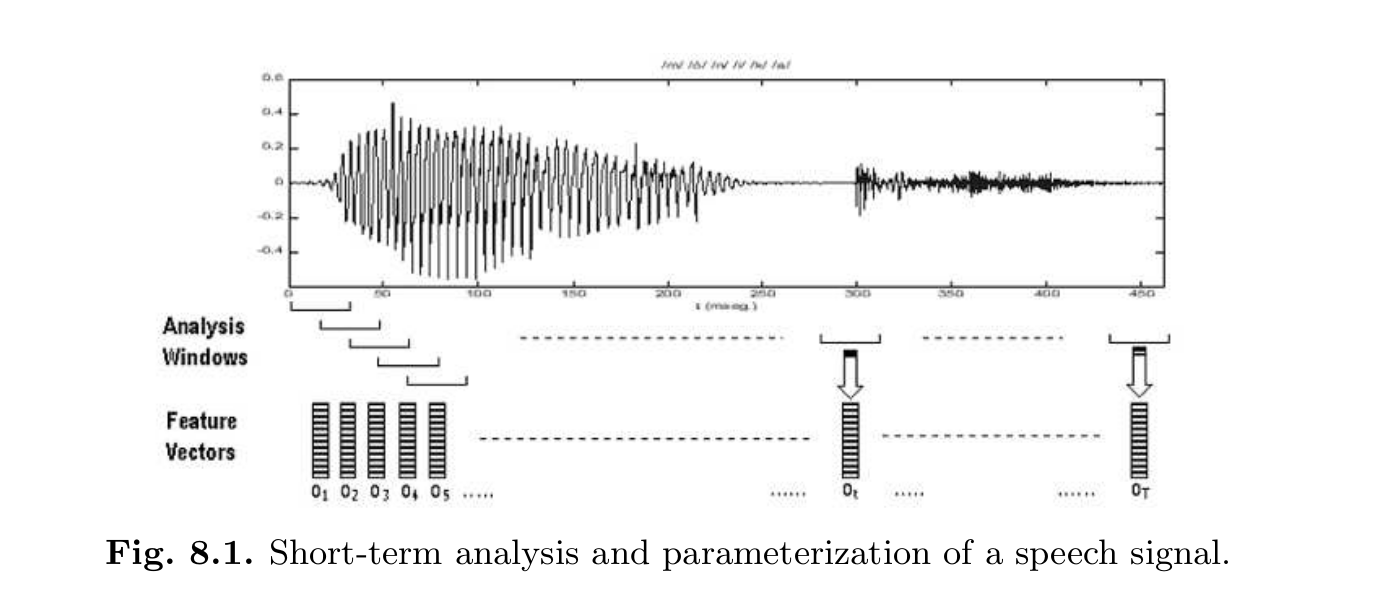
\includegraphics[width=0.9\linewidth]{images/figure_8_1.png}
		\caption{Handbook of Biometrics, page 155}
		\label{fig:writing-thesis}
	\end{figure}
\end{frame}

\begin{frame}{Tham số hóa}
	Tham số hóa bằng cách dùng Linear Predictive Coding (LPC)
	\begin{figure}[h!]
		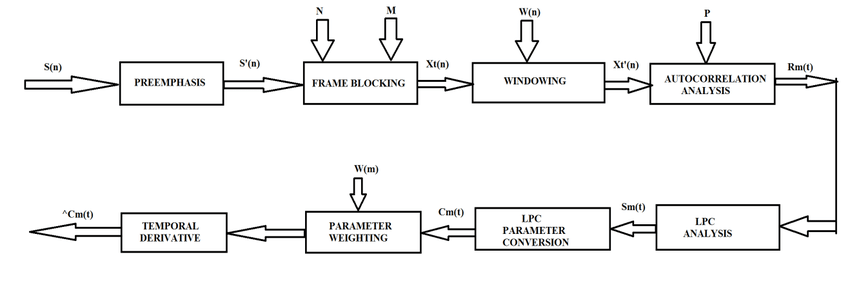
\includegraphics[width=0.9\linewidth]{images/Block-diagram-of-LPC-Linear-Predictive-Coding.png}
		\caption{Handbook of Biometrics, page 162}
		\label{fig:writing-thesis}
	\end{figure}
\end{frame}
\begin{frame}{Tham số hóa}
	Tham số hóa bằng cách dùng Mel-Frequency based Cepstral Coefficients (MFCC)
	\begin{figure}[H]
		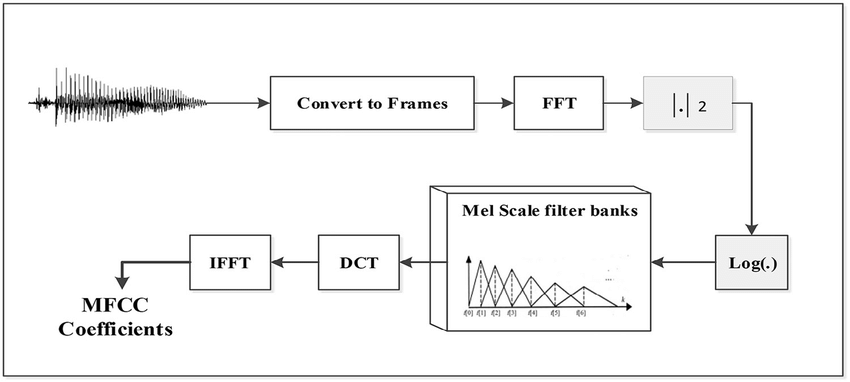
\includegraphics[width=0.9\linewidth]{images/Extraction-Mel-frequency-cepstral-coefficients-MFCC-from-the-audio-recording-signals.png}
		\caption{Handbook of Biometrics, page 162}
		\label{fig:writing-thesis}
	\end{figure}
\end{frame}
\begin{frame}{Phân tích ngữ âm và tách từ}
	Mô hình Hidden Markov
	\begin{figure}[h!]
		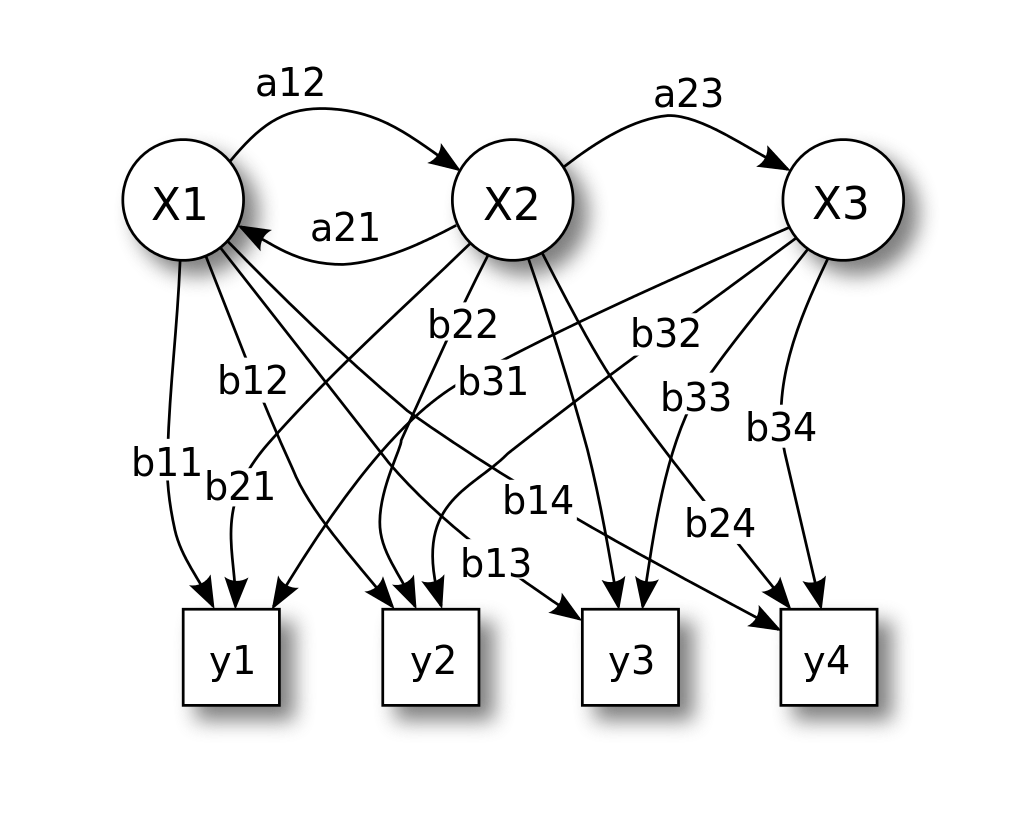
\includegraphics[width=0.6\linewidth]{images/1024px-HiddenMarkovModel.svg.png}
		\caption{Sơ đồ mô hình Markov ẩn}
		\label{fig:writing-thesis}
	\end{figure}
	
\end{frame}
\begin{frame}{Phân tách ngữ điệu}
	Dựa trên cơ sở là cao độ và năng lượng ở từng frame
	\begin{itemize}
		\item Cao độ: xác định bằng phương pháp tự động tương quan, phân rã cepstral dựa trên một số phương thức làm mịn bằng bộ lọc.
		\item Năng lượng: Năng lượng cửa sổ thu được rất dễ dàng thông qua định lý Parseval.
	\end{itemize}
\end{frame}

\subsection{Nhận dạng giọng nói phụ thuộc văn bản}
\begin{frame}{Giới thiệu}
	Hệ thống nhận dạng giọng nói phụ thuộc văn bản, sử dụng nội dung từ vựng của giọng nói phát
	ra để nhận dạng giọng nói, ứng dụng chính của hệ thống này trong các hệ thống tương tác, nơi cần có sự hợp tác từ người dùng để xác thực danh tính của họ.
	
	Phân loại
	\begin{itemize}
		\item Hệ thống văn bản tĩnh: nội dung từ vựng trong ghi danh và các mẫu nhận dạng luôn giống
		nhau.
		\item Hệ thống văn bản động: tạo ra một lời nhắc mật khẩu được tạo ngẫu nhiên khác nhau mỗi
		khi người dùng được xác minh (hệ thống nhắc bằng văn bản)
	\end{itemize}

	Kho ngữ liệu
	\begin{itemize}
		\item YOHO Speaker Verification
		\item MIT Mobile Device Speaker Verification Corpus
		\item BIOSEC Baseline Corpus
	\end{itemize}
\end{frame}
\begin{frame}{Phương pháp thực hiện}
	\begin{itemize}
		\item Phương pháp dựa trên khuôn mẫu: bao gồm một số chuỗi vectơ tương ứng với lời nói đăng
		ký và việc nhận dạng được thực hiện bằng cách so sánh lời nói xác minh với lời nói đăng ký.
		\item Phương pháp thống kê: Nổi bật nhất là mô hình Markov ẩn (HMM), cho phép chọn đơn vị tiếng nói từ đơn vị âm vị phụ đến từ và cho phép thiết kế hệ thống nhắc văn bản.
	\end{itemize}
\end{frame}
\begin{frame}{Công trình tiêu biểu}
	\begin{itemize}
		\item Introduction 1
		\item Introduction 2
		\item Introduction 3
	\end{itemize}
\end{frame}

\subsection{Nhận dạng giọng nói không phụ thuộc văn bản}
\begin{frame}{Giới thiệu}
	
\end{frame}
\begin{frame}{Hệ thống phổ âm trong thời gian ngắn}
	
\end{frame}
\begin{frame}{Hệ thống Idiolectal}

\end{frame}
\begin{frame}{Hệ thống ngữ âm}
	Mô hình hệ thống ngữ âm
	\begin{figure}[H]
		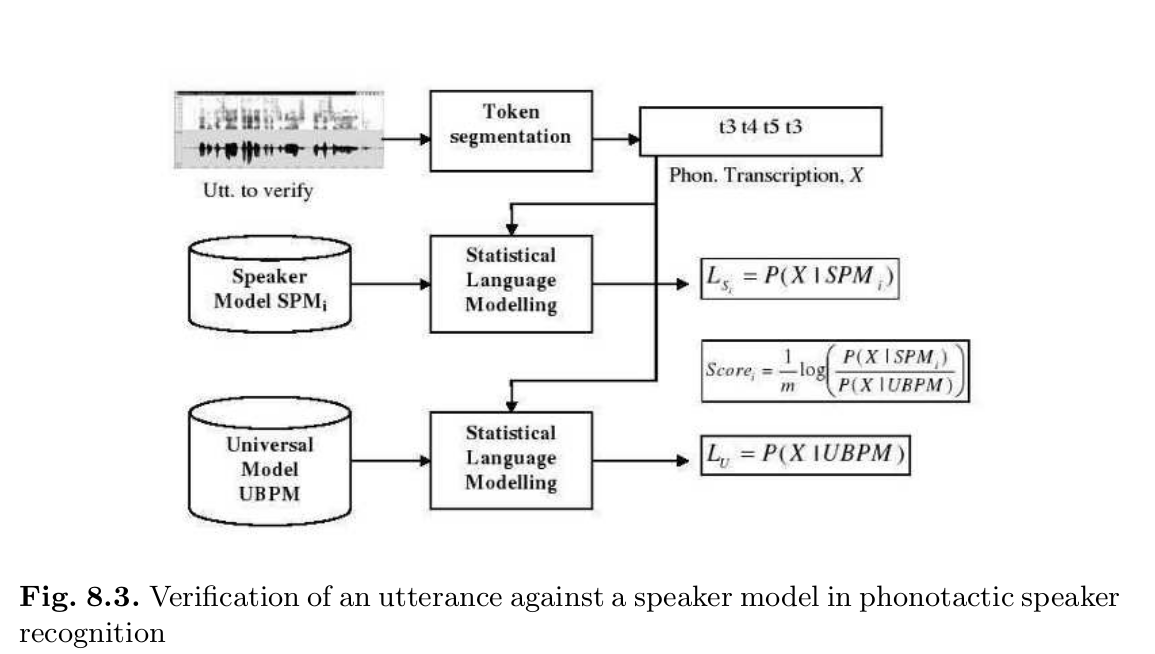
\includegraphics[width=0.9\linewidth]{images/figure_8_3.png}
		\caption{Handbook of Biometrics, page 162}
		\label{fig:writing-thesis}
	\end{figure}
\end{frame}	
\begin{frame}{Hệ thống ngữ điệu}
	Mô hình hệ thống ngữ điệu
	\begin{figure}
		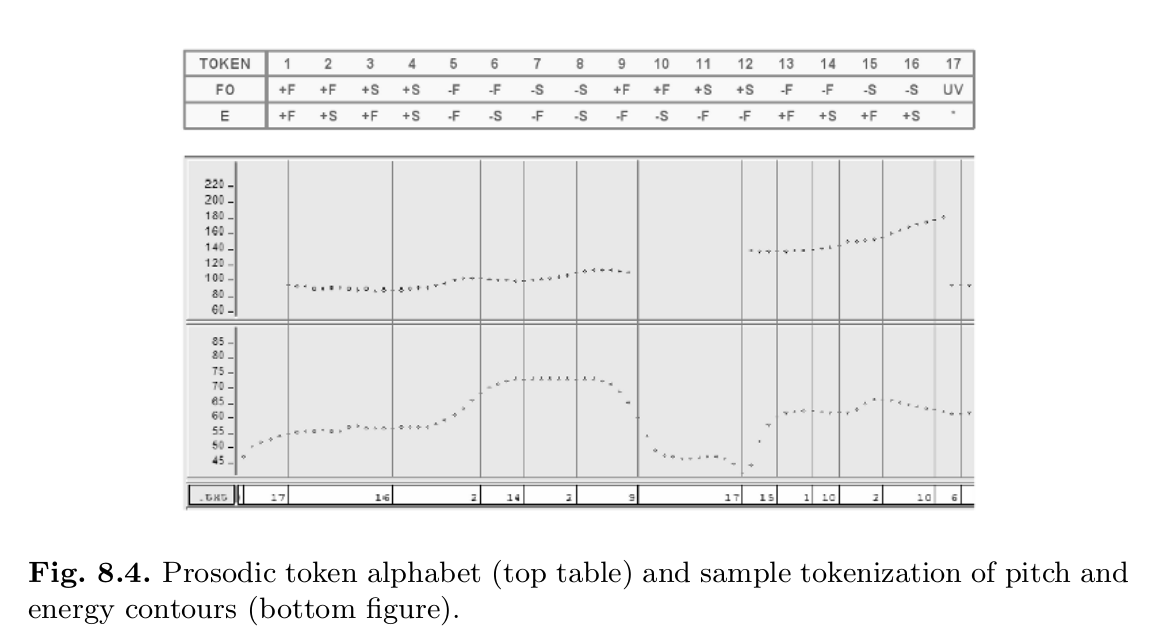
\includegraphics[width=0.9\linewidth]{images/figure_8_4.png}
		\caption{Handbook of Biometrics, page 163}
		\label{fig:writing-thesis}
	\end{figure}
\end{frame}	
\begin{frame}{Công trình tiêu biểu}
	\begin{itemize}
		\item Introduction 1
		\item Introduction 2
		\item Introduction 3
	\end{itemize}
\end{frame}

\subsection{Ứng dụng của nhận dạng giọng nói}
\begin{frame}{Voice authentication}
	\begin{figure}[h!]
		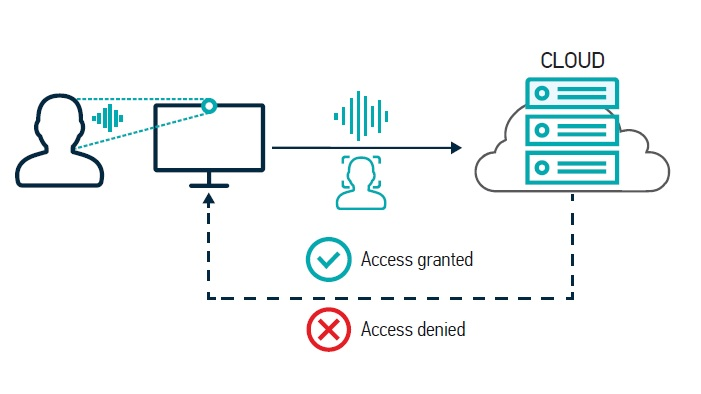
\includegraphics[width=0.9\linewidth]{images/voice_authentication.jpg}
		\caption{Ví dụ Voice authentication/ Verification}
		\label{fig:writing-thesis}
	\end{figure}
\end{frame}	
\begin{frame}{Speaker Identification and Verification}
	\begin{figure}[H]
		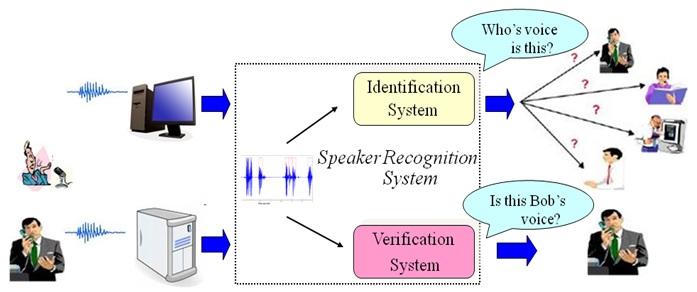
\includegraphics[width=0.9\linewidth]{images/speaker_identification_verification.jpeg}
		\caption{Ví dụ Speaker Recognition Systems}
		\label{fig:writing-thesis}
	\end{figure}
\end{frame}
\begin{frame}{Forensic speaker recognition}
	\begin{figure}[H]
		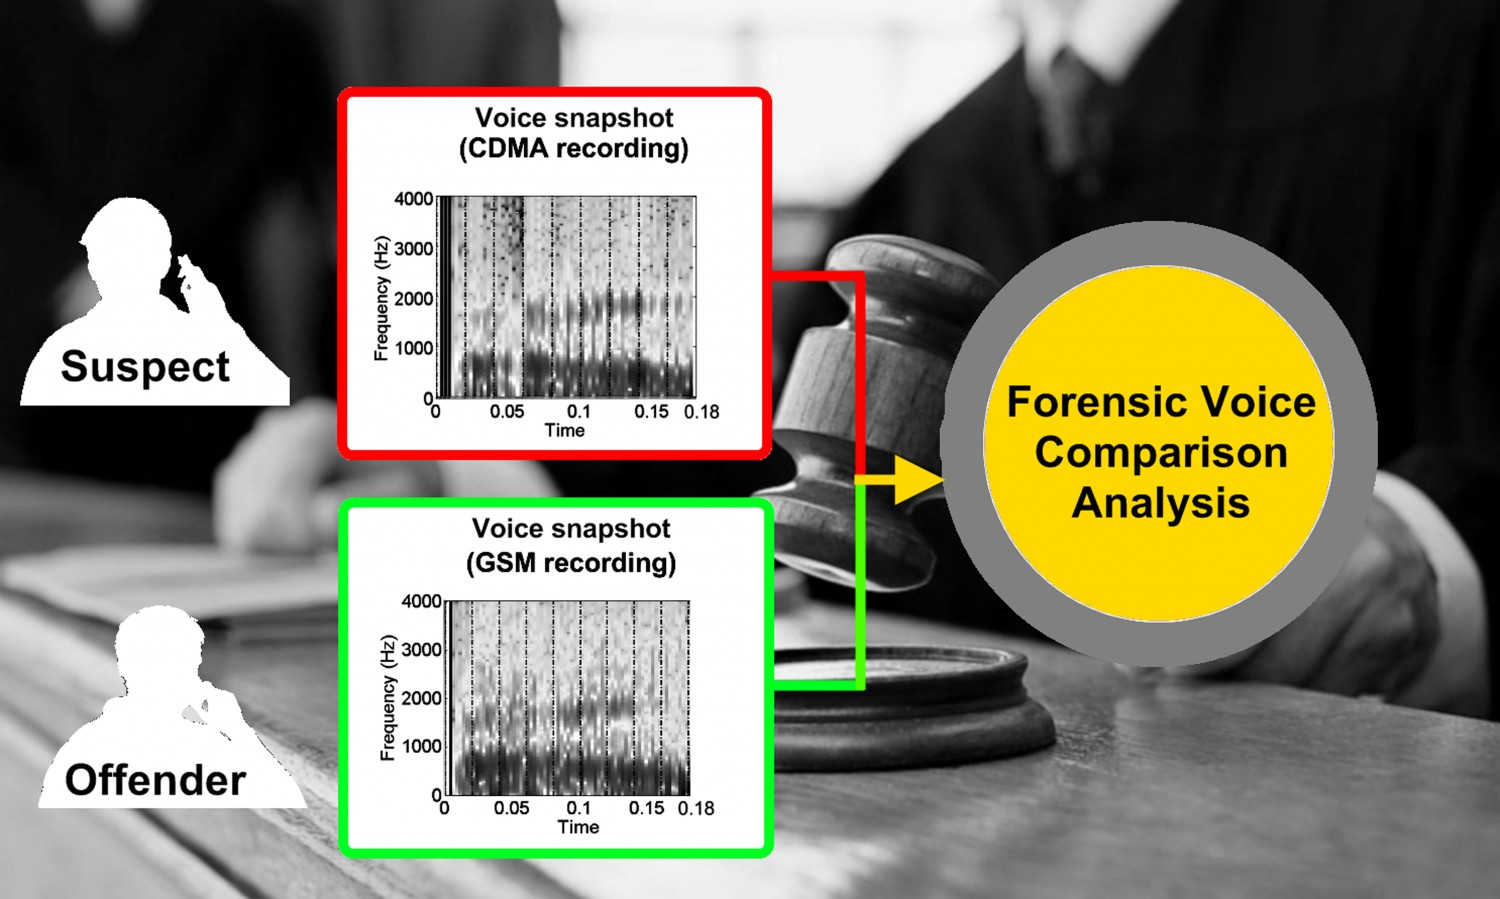
\includegraphics[width=0.9\linewidth]{images/forensic_voice.jpg}
		\caption{Ví dụ Speaker Recognition Systems}
		\label{fig:writing-thesis}
\end{figure}
\end{frame}

\section{Các phương pháp SOTA - Voice Biometrics}
\subsection{Động lực nghiên cứu khoa học}
\begin{frame}{Động lực nghiên cứu khoa học}
		\begin{itemize}
		\item Những phương pháp đã tìm hiểu từ sách Handbook of Biometrics: Voice Biometrics đã cho chúng ta cái nhìn tổng quan về lĩnh vực Nhận dạng giọng nói và những phương pháp truyền thống (tạm gọi là thời kỳ trước Deep Learning) cùng với những thông tin các công trình nghiên cứu nổi bật.
		\item Các phương pháp SOTA dựa trên việc biểu diễn i-vectors của những
		đoạn giọng nói, cải thiện đáng kể so với mô hình Gaussian Mixture
		Model-Universal Background Models
		\item Sự phát triển của Deep Learning
	\end{itemize}
\end{frame}
\subsection{Phát biểu bài toán}
\begin{frame}{Phát biểu bài toán}
	\textbf{Tác vụ:} Định danh người nói
	\begin{itemize}
		\item Đầu vào (Input): Dữ liệu âm thanh giọng nói
		\item Đầu ra (Output): Danh tính của người nói
	\end{itemize}
	\textbf{Tác vụ:} Xác nhận người nói
	\begin{itemize}
		\item Đầu vào (Input): Dữ liệu âm thanh giọng nói
		\item Đầu ra (Output): Đồng ý/ Từ chối
	\end{itemize}
\end{frame}
\subsection{Các công trình liên quan}
\begin{frame}{Công trình tiêu biểu sử dụng d-vectors}
	Mô hình d-vectors
	\begin{figure}[H]
		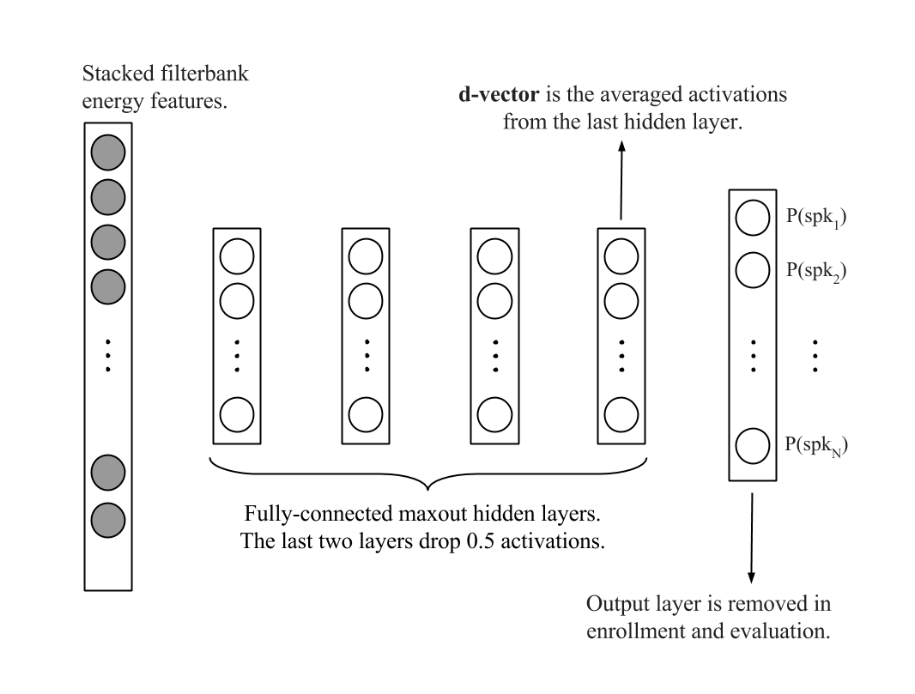
\includegraphics[width=0.7\linewidth]{images/d-vectors.png}
		\caption{Mô hình DNN với d-vectors}
		\label{fig:writing-thesis}
	\end{figure}
\end{frame}
\begin{frame}{Công trình tiêu biểu sử dụng d-vectors}
	Giới thiệu về công trình: Speaker Recognition from raw waveform with SincNet
\end{frame}
\begin{frame}{Công trình tiêu biểu sử dụng d-vectors}
	Phương pháp tiếp cận
\end{frame}
\begin{frame}{Công trình tiêu biểu sử dụng d-vectors}
	Kết quả đạt được
\end{frame}
\begin{frame}{Công trình tiêu biểu sử dụng j-vectors}
	Mô hình j-vectors
	\begin{figure}[H]
		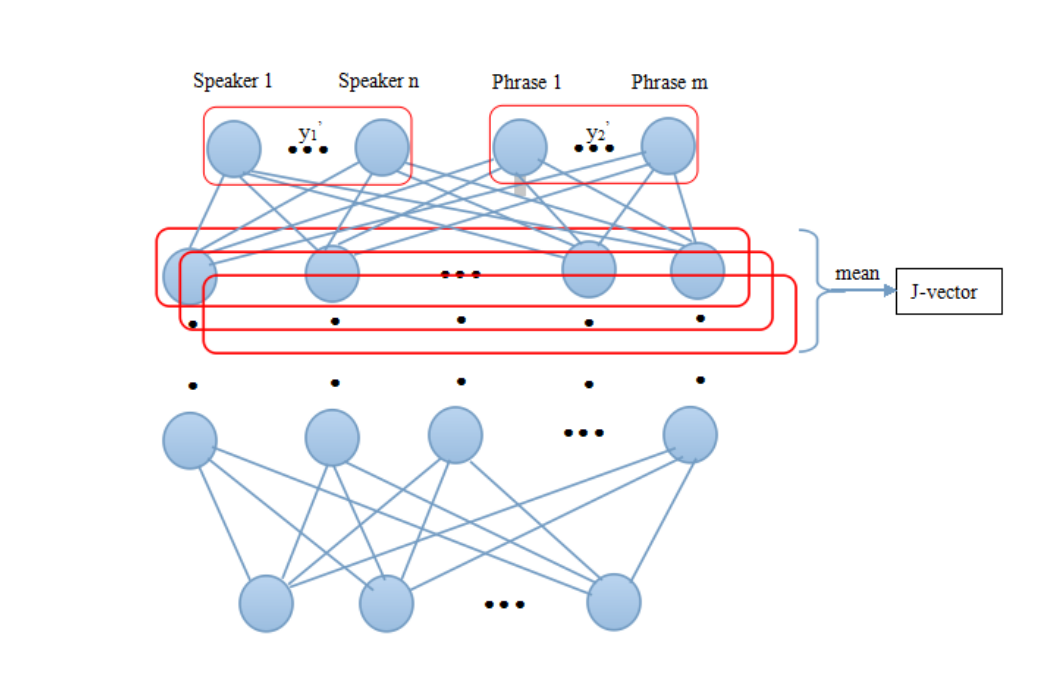
\includegraphics[width=0.7\linewidth]{images/j-vectors.png}
		\caption{Mô hình DNN với j-vectors}
		\label{fig:writing-thesis}
	\end{figure}
\end{frame}
\begin{frame}{Công trình tiêu biểu sử dụng j-vectors}
	Giới thiệu về công trình
\end{frame}
\begin{frame}{Công trình tiêu biểu sử dụng j-vectors}
	Phương pháp tiếp cận
\end{frame}
\begin{frame}{Công trình tiêu biểu sử dụng j-vectors}
	Các kết quả đạt được
\end{frame}
\begin{frame}{Công trình tiêu biểu sử dụng x-vectors}
	Mô hình x-vectors
	\begin{figure}[H]
		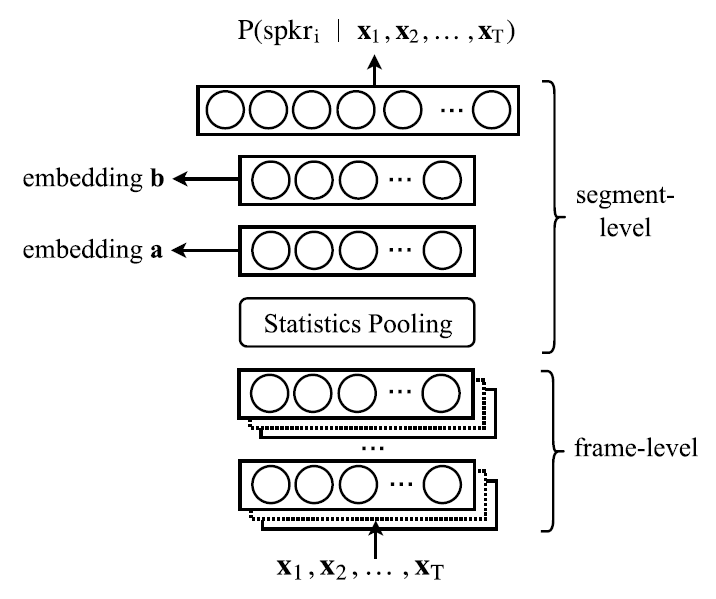
\includegraphics[width=0.65\linewidth]{images/x-vector.jpg}
		\caption{Mô hình DNN với x-vectors}
		\label{fig:writing-thesis}
	\end{figure}
\end{frame}
\begin{frame}{Công trình tiêu biểu sử dụng x-vectors}
	Giới thiệu về công trình
\end{frame}
\begin{frame}{Công trình tiêu biểu sử dụng x-vectors}
	Phương pháp
\end{frame}
\begin{frame}{Công trình tiêu biểu sử dụng x-vectors}
	Các kết quả đạt được
\end{frame}
\begin{frame}{So sánh d-vectors, j-vectors và x-vectors}
	
\end{frame}
\subsection{Thực nghiệm}
\begin{frame}{Thực nghiệm}
\end{frame}
\subsection{Tài liệu tham khảo - References}
\begin{frame}
	\nocite{*}
	\bibliography{references}\newpage\cleardoublepage
	\bibliographystyle{plain}
\end{frame}

\end{document}